% --- UC1: User Registration ---
\subsubsection*{[UC1] User Registration Sequence Diagram}
\begin{figure}[H]
    \centering
    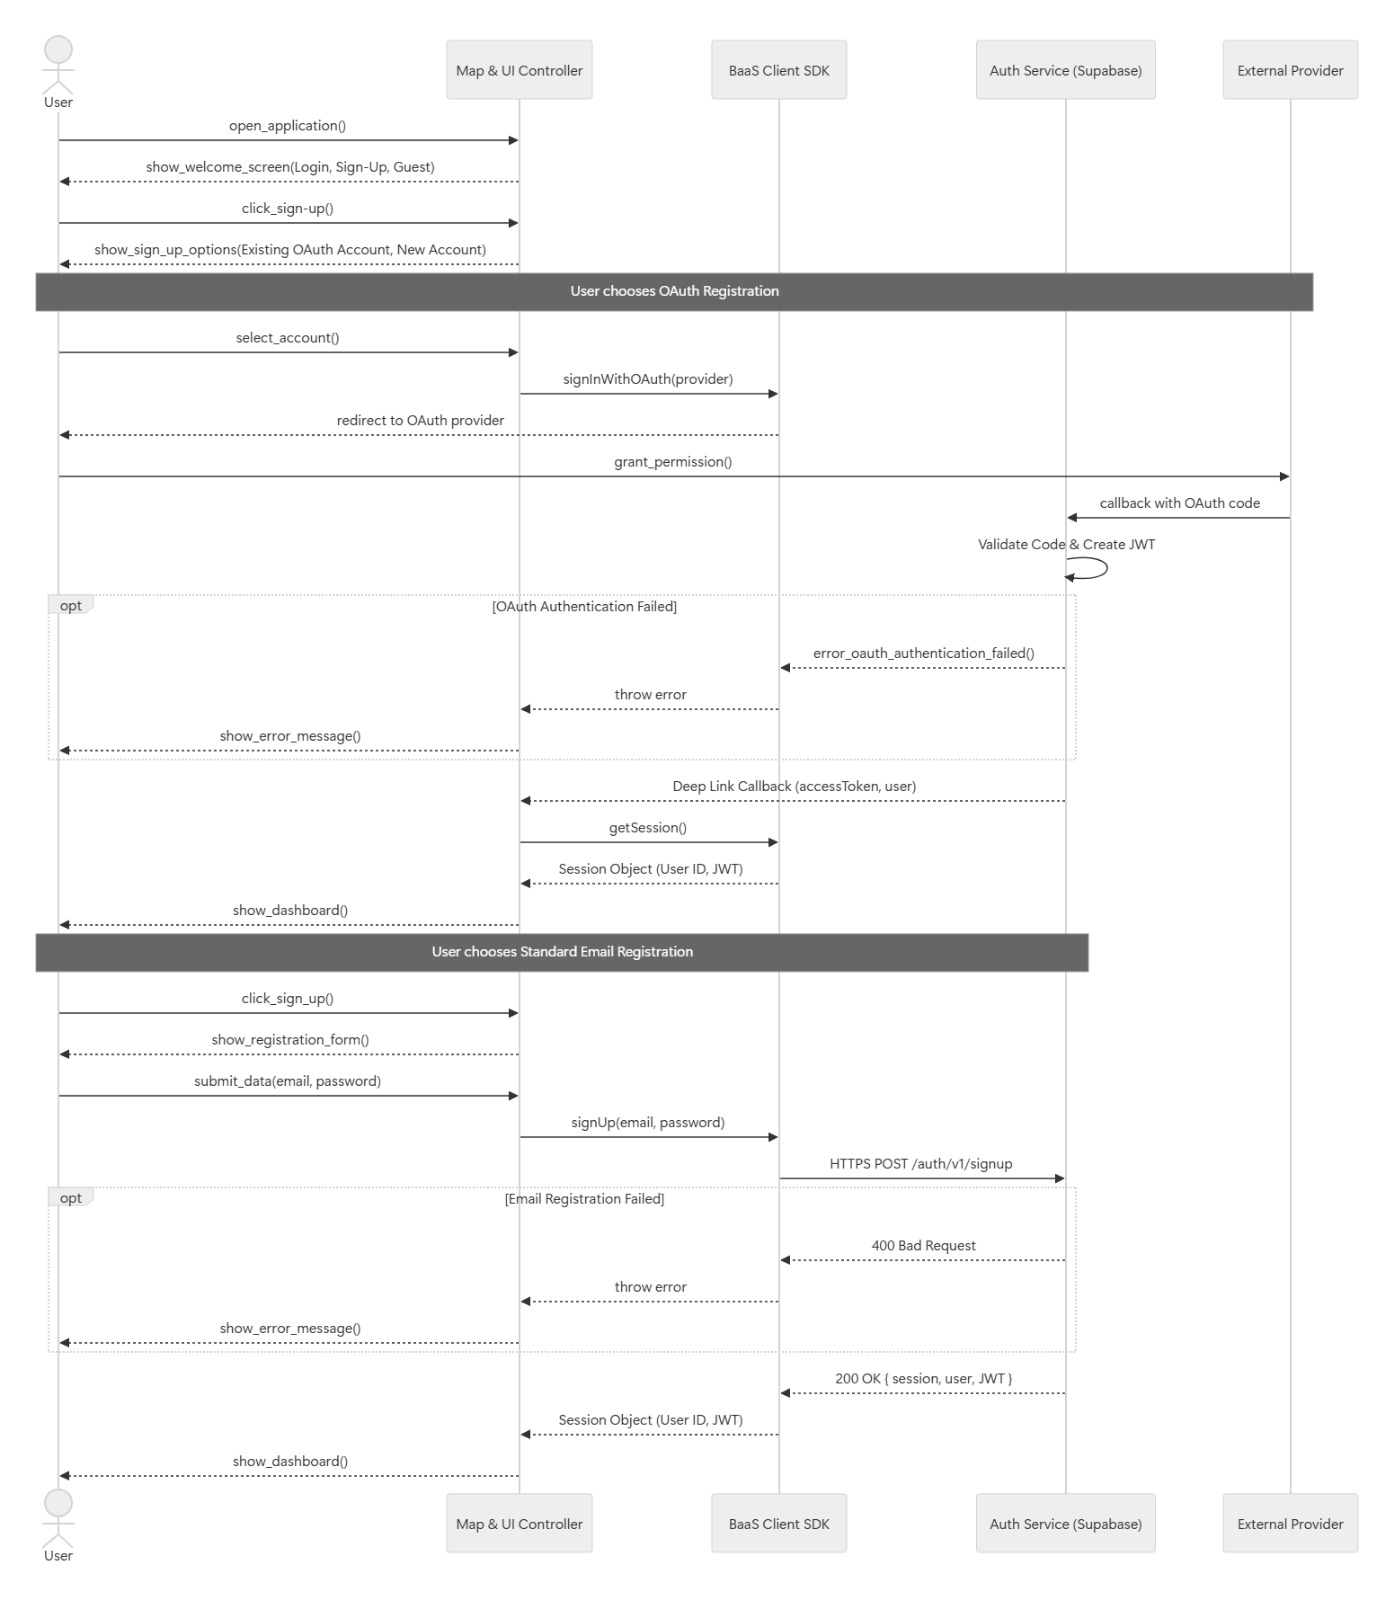
\includegraphics[width=\textwidth]{Images/uc1_sd.jpeg}
    \caption{[UC1] User Registration Sequence Diagram}
    \label{fig:sd_uc1}
\end{figure}
The diagram illustrates the registration process managed by the Auth Service. In the OAuth scenario, the flow delegates authentication to the external provider via redirect and callback (Deep Link). In the Email scenario, the SDK communicates directly with the Supabase API. In both cases, the final result is the acquisition of a valid JWT (JSON Web Token), which is essential for ensuring secure access to the database via RLS policies in subsequent interactions.

% --- UC2: System Access ---
\subsubsection*{[UC2] System Access Sequence Diagram}
\begin{figure}[H]
    \centering
    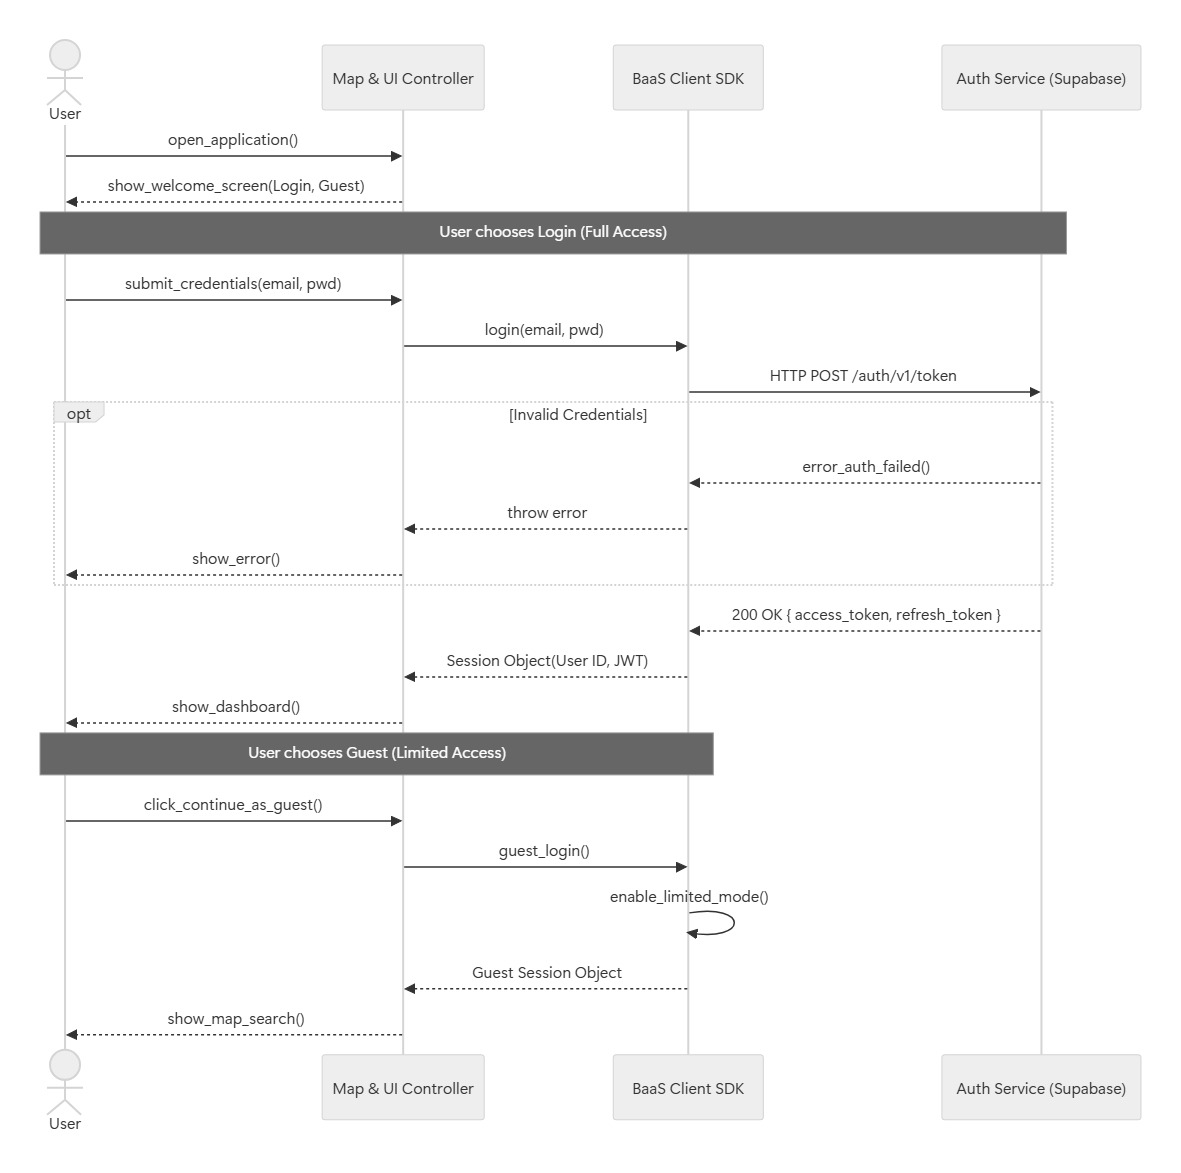
\includegraphics[width=\textwidth]{Images/uc2_sd.jpeg}
    \caption{[UC2] System Access Sequence Diagram}
    \label{fig:sd_uc2}
\end{figure}
This diagram depicts the session negotiation process. For registered users, the BaaS Client SDK exchanges credentials for a persistent session token. For Guest users, the SDK initializes a local session in "Limited Mode," which disables write calls to the database and restricts access exclusively to public search APIs.

% --- UC3: Activity Recording ---
\subsubsection*{[UC3] Activity Recording Sequence Diagram}
\begin{figure}[H]
    \centering
    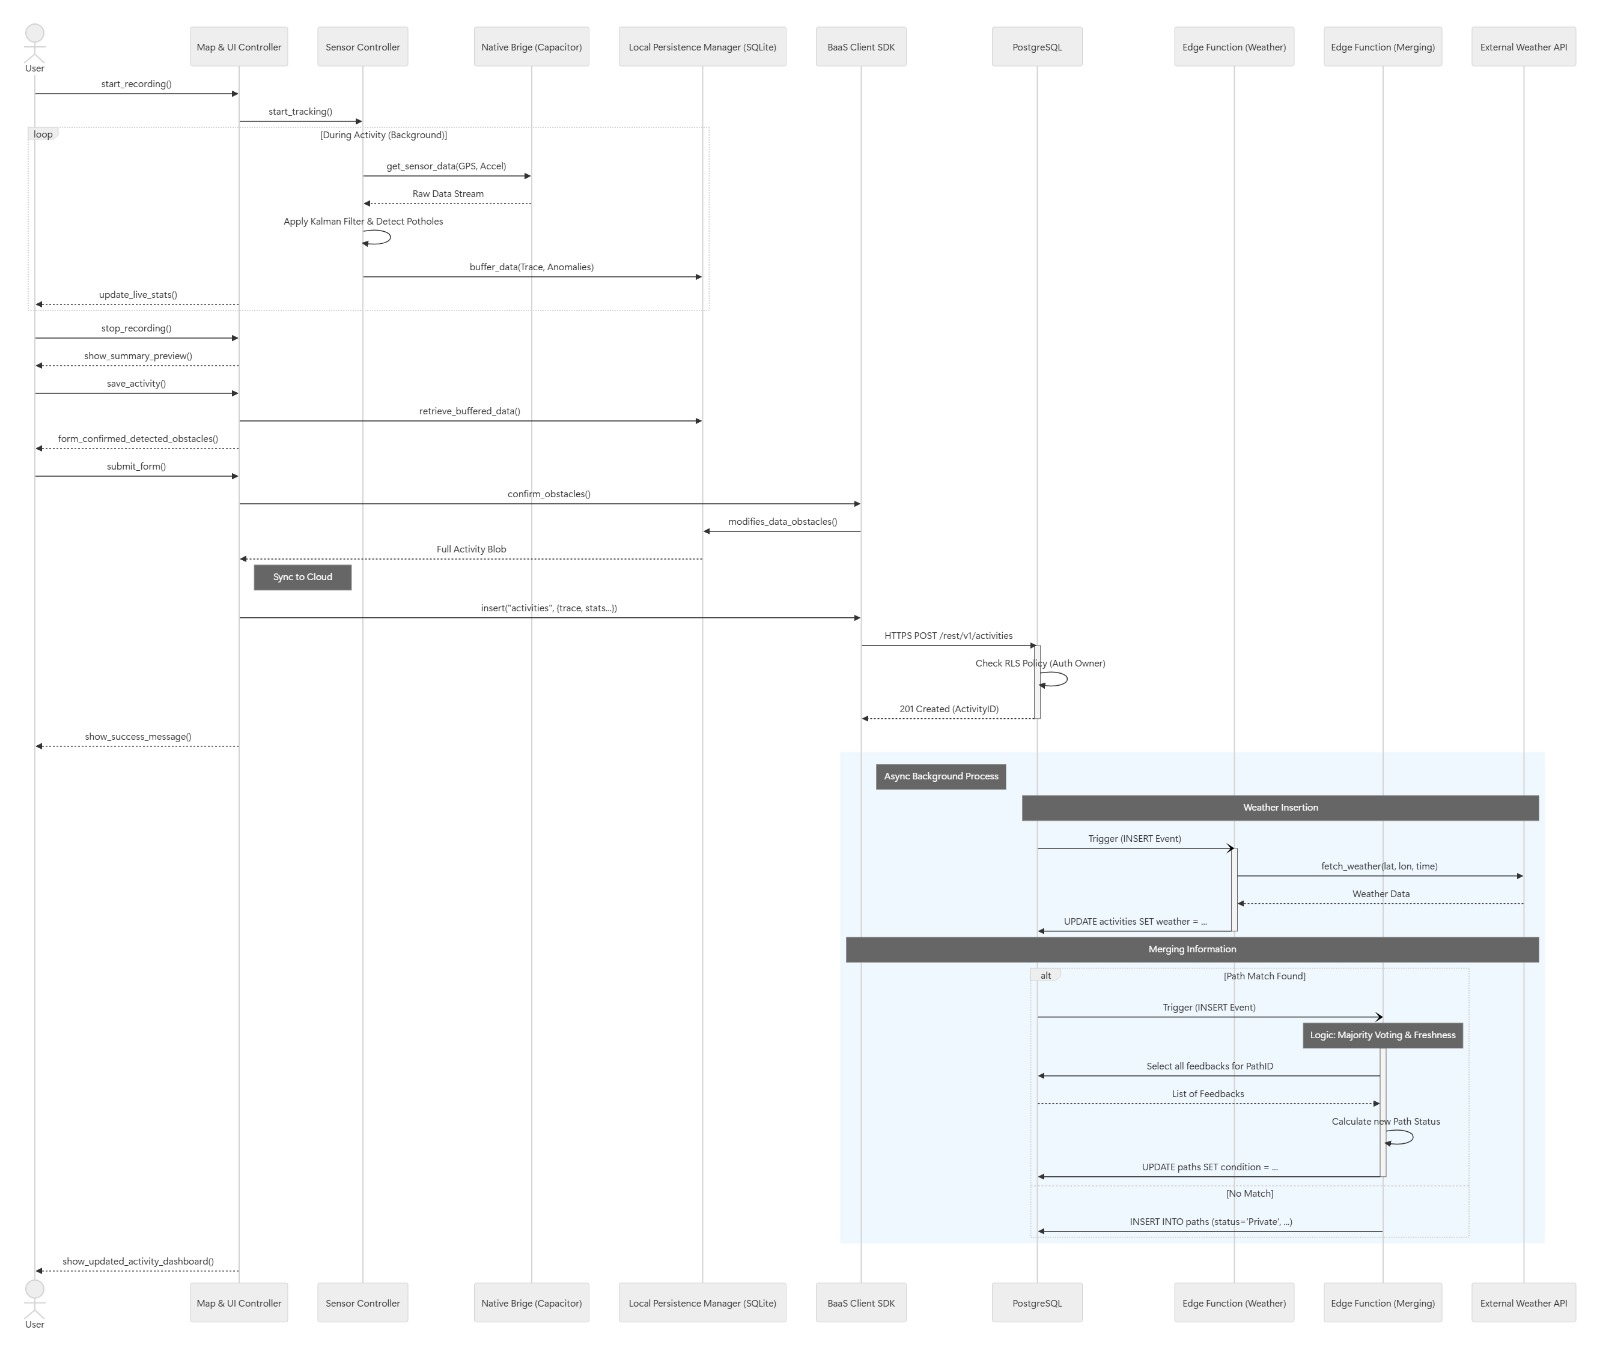
\includegraphics[width=\textwidth]{Images/uc3_sd.jpeg}
    \caption{[UC3] Activity Recording Sequence Diagram}
    \label{fig:sd_uc3}
\end{figure}
The diagram highlights the Thick Client and Offline-First architecture. Data acquisition is performed via the Native Bridge, filtered, and saved locally on SQLite. Synchronization with the Cloud triggers asynchronous processes (Serverless): meteorological enrichment and the Merging logic. Note that the trace comparison logic occurs entirely server-side (Edge Function) to avoid burdening the user device and to guarantee data consistency.

% --- UC4: Creation of a manual path ---
\subsubsection*{[UC4] Creation of a manual path Sequence Diagram}
\begin{figure}[H]
    \centering
    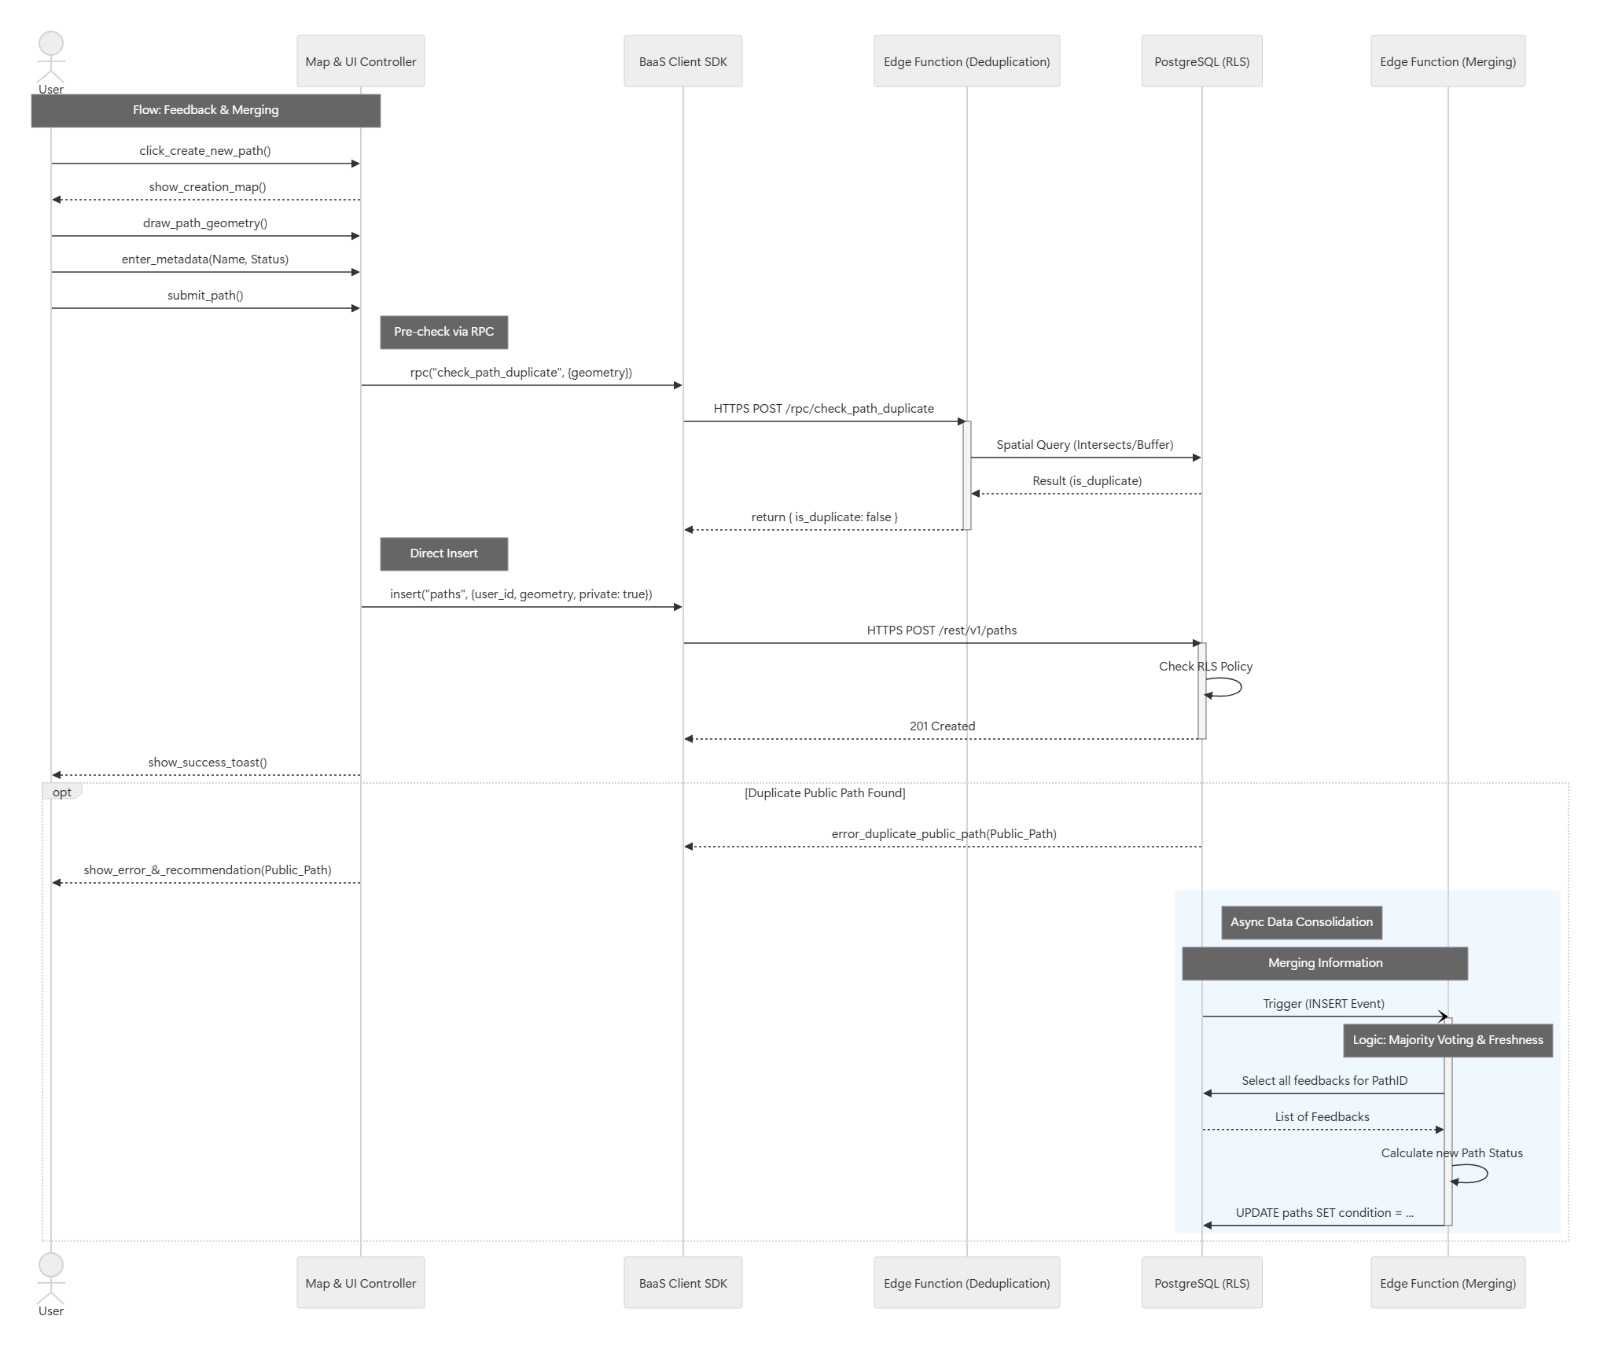
\includegraphics[width=\textwidth]{Images/uc4_sd.jpeg}
    \caption{[UC4] Creation of a manual path Sequence Diagram}
    \label{fig:sd_uc4}
\end{figure}
This scenario illustrates the hybrid interaction between direct DB calls and server-side logic. Before inserting the path, the client invokes a Remote Procedure Call (RPC) on a specific Edge Function (Deduplication) to verify the existence of duplicate paths via complex spatial queries (PostGIS). If the check passes, the client proceeds with direct insertion into the database; otherwise, it merges the information entered by the user into the existing public path that corresponds to the inserted geometry.

% --- UC5: Publication of a path ---
\subsubsection*{[UC5] Publication of a path Sequence Diagram}
\begin{figure}[H]
    \centering
    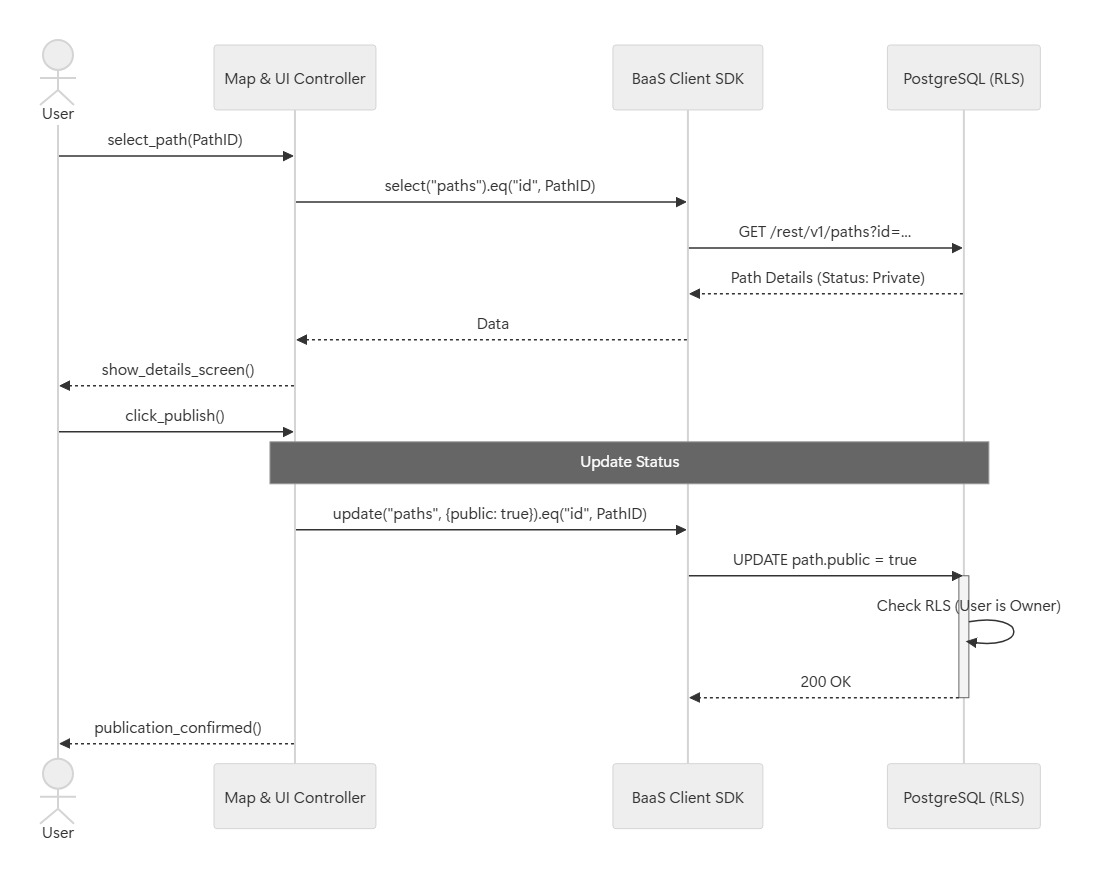
\includegraphics[width=\textwidth]{Images/uc5_sd.jpeg}
    \caption{[UC5] Publication of a path Sequence Diagram}
    \label{fig:sd_uc5}
\end{figure}
This represents the state transition of a path from Private to Public. The operation is a direct UPDATE call via the SDK. Security is guaranteed by the PostgreSQL database engine, which, through RLS policies, verifies that the request author corresponds to the record owner before applying the modification.

% --- UC6: Path Feedback reporting ---
\subsubsection*{[UC6] Path Feedback reporting Sequence Diagram}
\begin{figure}[H]
    \centering
    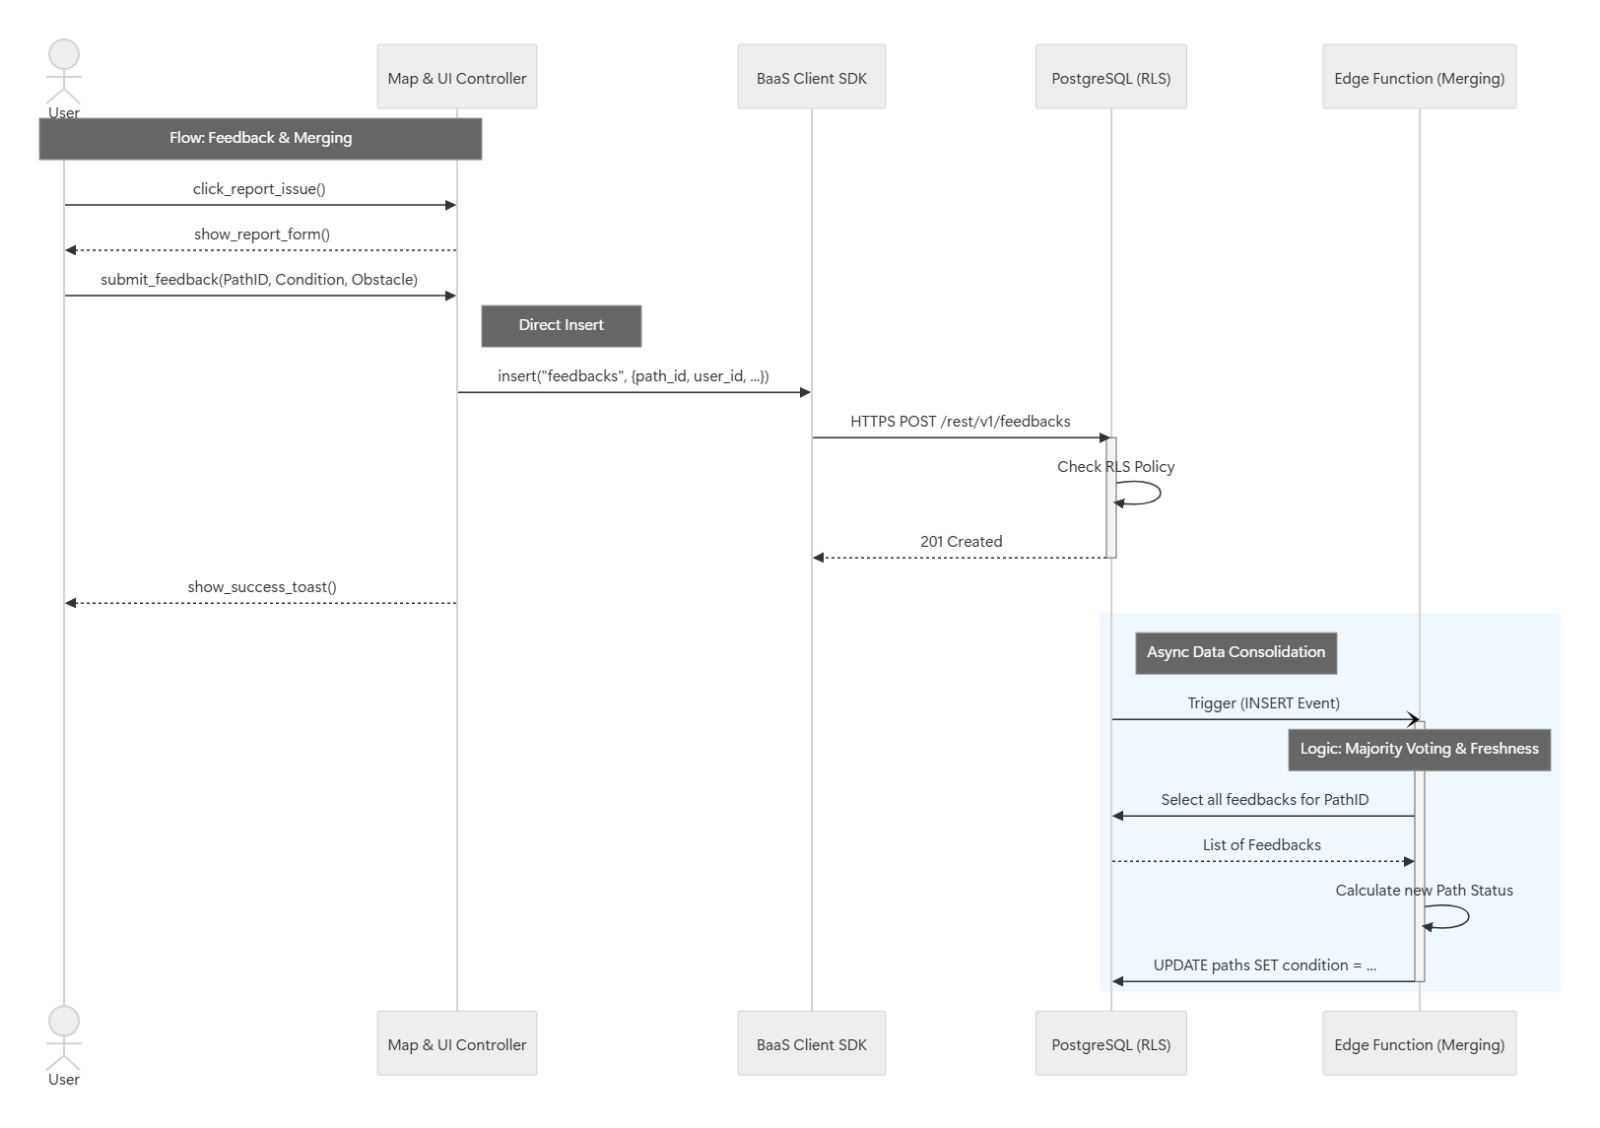
\includegraphics[width=\textwidth]{Images/uc6_sd.jpeg}
    \caption{[UC6] Path Feedback reporting Sequence Diagram}
    \label{fig:sd_uc6}
\end{figure}
The diagram demonstrates the Event-Driven architecture. The client handles only the rapid insertion of the feedback to ensure user responsiveness. The database emits an internal event (Trigger) that asynchronously activates the Merging Edge Function. This function recalculates the path status by aggregating existing feedbacks according to the "Majority Voting" algorithm defined in the RASD.

% --- UC7: Search for a path ---
\subsubsection*{[UC7] Search for a path Sequence Diagram}
\begin{figure}[H]
    \centering
    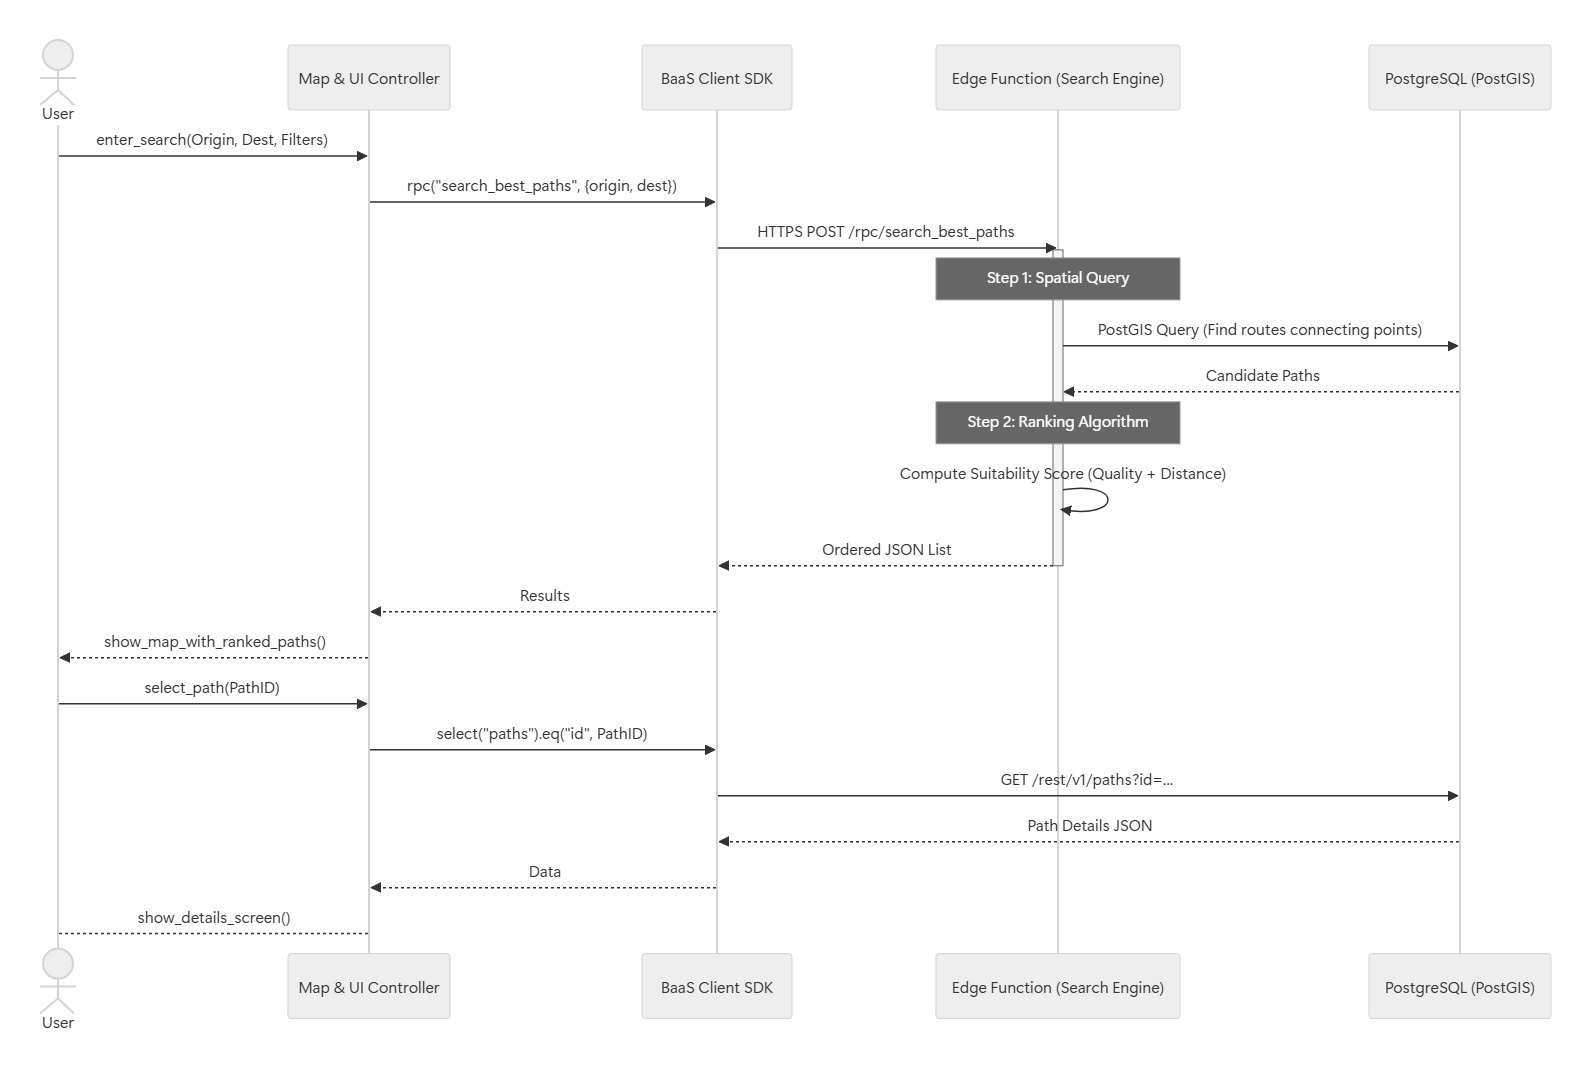
\includegraphics[width=\textwidth]{Images/uc7_sd.jpeg}
    \caption{[UC7] Search for a path Sequence Diagram}
    \label{fig:sd_uc7}
\end{figure}
Since the ranking algorithm requires complex calculations (combining geometric distance and quality score), the search is not a simple DB query but is encapsulated in an RPC (Remote Procedure Call). The Edge Function executes the spatial query on PostGIS and sorts the results in memory before returning them to the client, optimizing performance and reducing data traffic.
